%
% Modified by Megan Patnott
% Last Change: Jan 18, 2013
%
%%%%%%%%%%%%%%%%%%%%%%%%%%%%%%%%%%%%%%%%%%%%%%%%%%%%%%%%%%%%%%%%%%%%%%%%
%
% Modified by Sameer Vijay
% Last Change: Tue Jul 26 2005 13:00 CEST
%
%%%%%%%%%%%%%%%%%%%%%%%%%%%%%%%%%%%%%%%%%%%%%%%%%%%%%%%%%%%%%%%%%%%%%%%%
%
% Sample Notre Dame Thesis/Dissertation
% Using Donald Peterson's ndthesis classfile
%
% Written by Jeff Squyres and Don Peterson
%
% Provided by the Information Technology Committee of
%   the Graduate Student Union
%   http://www.gsu.nd.edu/
%
% Nothing in this document is serious except the format.  :-)
%
% If you have any suggestions, comments, questions, please send e-mail
% to: ndthesis@gsu.nd.edu
%
%%%%%%%%%%%%%%%%%%%%%%%%%%%%%%%%%%%%%%%%%%%%%%%%%%%%%%%%%%%%%%%%%%%%%%%%


%
% Chapter 2
%

\chapter{Future Work}

\section{Detector Upgrades}

\subsection{Magnet Designs}

\subsection{FIREBALL}

\section{Target Upgrades}

One of the concerns and limitations of the original experiments was the thickness of the target. Ideally, the target being used would be less that 500 $\mu g/cm^2$, but the ones used were 1.7 $mg/cm^2$ and 1.44 $mg/cm^2$. While these targets were self-supporting, they were thick enough that electron straggling occurred, smearing out the spectrum.

To create a thinner target, it was decided to try and use a carbon-backing. The Sm was then evaporated onto the backing. The carbon was 20 $\mu g/cm^2$. In the targets made, the Sm was measured to be 170 $\mu g/cm^2$, ten times thinner than the original targets used.

To compare the old and new targets, an experiment was run with both targets inside of ICEBall. 

The new targets could be run with higher beam currents to get similar rates in the detectors, at what appeared to be a proportional rate to the target thickness.

At lower electron energies, the carbon-backed targets had far better resolution, as seen in Figure \ref{fig:target_test}.

\begin{figure}
    \centering
    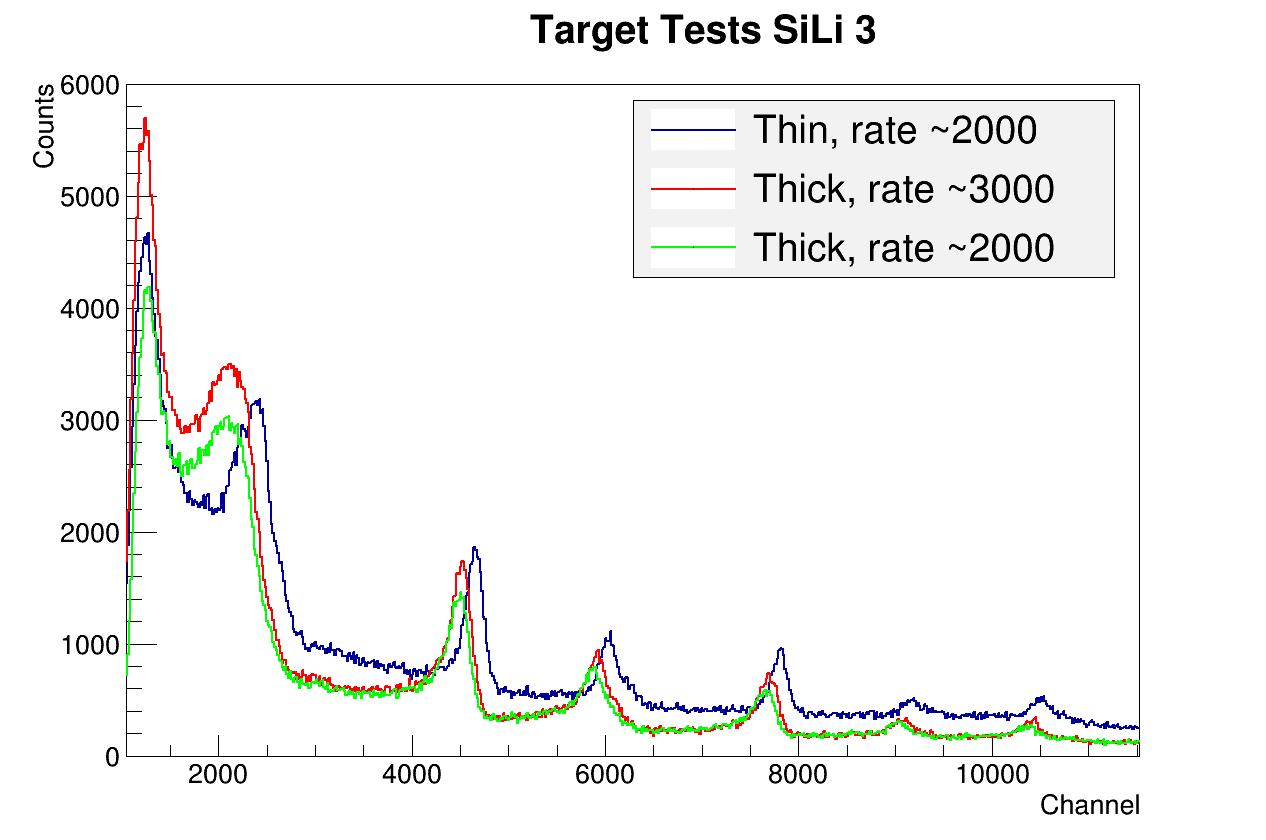
\includegraphics{Future_Figs/SiLi3.png}
    \caption{Comparison of the thick (self-supporting) and thin (carbon-backed) targets. The spectra were taken during the same experiment. At low energies, the resolution is better in the thin target. Further, the energies of the peaks shift based on which target it is.}
    \label{fig:target_test}
\end{figure}

\section{Alternative Reactions}

% % uncomment the following lines,
% if using chapter-wise bibliography
%
% \bibliographystyle{ndnatbib}
% \bibliography{example}
